\section{Evaluation}
~

\subsection{Environment setting}
~

The evaluation of the model is focused on two metrics : the makespan and the computing time once trained.
For the implementation of the model, python 3.10.12 with the PyTorch 2.4.1 library is used and runs on a google collab runtime
with 90 TPU cores.
The stochastic gradient descent is used for training with a learning rate of $0.001$ and a batch size of 250.

During the initial evaluation, an oversmoothing problem occured which lead to reducing the number of GCN layers to 1(see Section \ref{sec:model_design}).
Unfortunately reducing the number of GCN layers wasn't enough which lead 
to adding a regularization term to the loss function.
The idea is to tackle the over-smoothing probblem by forcing the model
to differentiate between the nodes' representation.
Hence, the regularization term is the squared inverse of the average euclidian distance 
between each of the nodes' latent representation, i.e., 
\begin{equation}
    \text{regTerm}(X) = \frac{1}{\sum_{i}\sum_{j > i} \Vert X_i - X_j\Vert_{2} }
\end{equation}
    
and the loss function then becomes
\begin{equation}
    loss(X, y) = \sum_{i} -y_i\log(x_i) + \text{regTerm}(X)
\end{equation}
with $x_i$ being the elements in $x$, the flattened matrix representation of $X$
and $y$ the true output (see Section \ref{sec:loss_design}).

\subsection{Dataset generation}
~

To generate the DAG tasks, the generator from \citet{zhao2020DAGsched} is used, which is also the one used in \citet{Lee2021GlobalDagSchedDRL}.
The random DAGs are generated using the following process :
The generator starts at a source node and expands outward, 
creating nodes in successive layers. The total number of layers, 
or maximum depth, is randomly determined to be between two values $a$ and $b$.
For each layer, the number of nodes generated is chosen uniformly, 
ranging from 2 up to the parallelism parameter, $p$ which in this case, 
is fixed at $p=8$. Nodes that do 
not already have connections can randomly connect to other nodes in 
the previous layer with a probability of $p_c=0.5$. After all layers 
are generated, any terminal nodes are linked to a final sink node. 
Both the source and sink nodes are used to structure the graph and 
have a fixed execution time of one unit each. Lastly, 
execution times are assigned randomly to all nodes while ensuring 
that the total workload sums up to $W = 1000$\cite{zhao2020DAGsched}.

To generate DAGs with a fixed number of nodes $n$, 
the generator is first used to generate 50000 DAG tasks
with different values for $a$ and $b$ depdending on what 
the value of $n$ is. Then, the generated DAGs with 
the specified number of nodes are retrieved from the dataset.
Specifically, Table \ref{tab:layer_num_minmax} 
shows the different $a$ and $b$ values according to $n$.

\begin{table}
    \centering
    \begin{tabular}{|c|c|c|}    
        \hline
        \textbf{n} & \textbf{a} & \textbf{b} \\
        \hline
        10 & 3 & 8 \\
        \hline
        \{20, 30\} & 5 & 8 \\
        \hline
        40 & 7 & 10 \\
        \hline
        50 & 10 & 15 \\
        \hline
    \end{tabular}
    \caption{dag generator $a$, minimum number of layers, and $b$, maximum
    number of layers, parameter values for generating 
    random DAGs according to number of fixed nodes per graph we need to retrieve afterwards.}
    \label{tab:layer_num_minmax}
\end{table}

Using those values, 1400 DAG tasks were retrieved and used for 
evaluation, for each value of $n$.
1000 of them were used for training the model, 400 for testing
and 100 of them were used to measure the computing time 
for both the ILP and the supervised ML methods.


\subsection{Computing time results}
~

The computing time for the ILP method is shown 
in Figure \ref{fig:ilp_compute_time}.
The ILP solver was timed out whenever the computing time exceeded 1 hour
and it did time out when considering systems of 2 and 4 cores, when the number of nodes
exceeded 20 nodes (i.e., 30, 40 and 50 nodes) per DAG task.
Hence, in the next sections, only 6 and 8 cores will be considered,
with the number of nodes not exceeding 30 nodes, to have enough
ILP solved DAGs for training the model. 

\begin{figure}
    \centering
    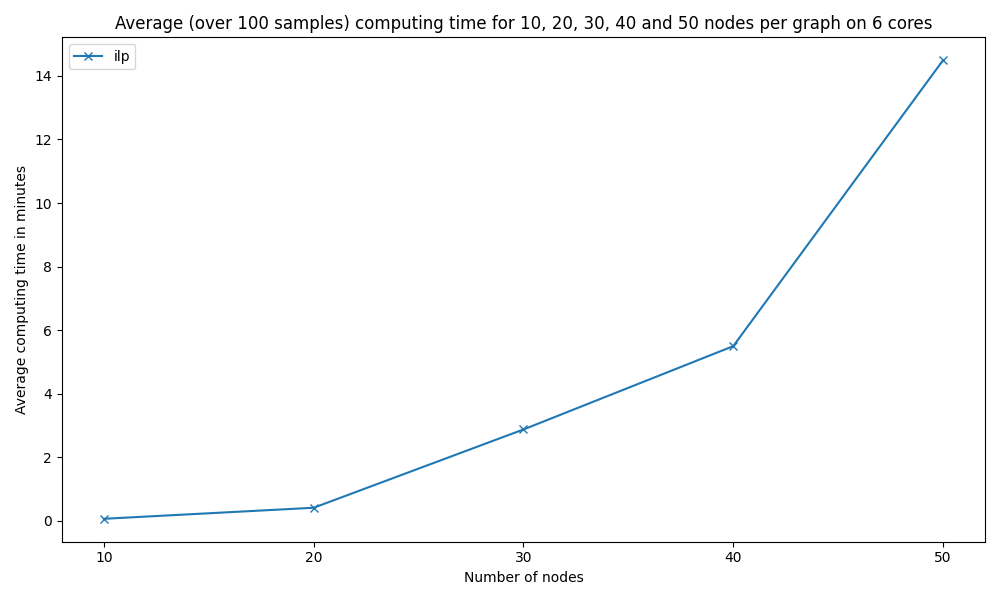
\includegraphics[width=\linewidth]{images/result_computing_time_ilp_m6.png}
    \caption{Average computing time for computing the optimal schedule
    of a single DAG task using the ILP method, in minutes, according to 
    the number of nodes in the DAG, on a system with 6 cores.}
    \label{fig:ilp_compute_time}
\end{figure}

As you can see from Figure \ref{fig:ilp_compute_time}, the more nodes there are on the system, 
the more time it takes for the ILP solver to compute the optimal schedule,
and it does so in, what it seems to be, an exponential growth.
Figure \ref{fig:ilp_compute_time} thus shows the non-scalability
of the ILP method, with the number of nodes per DAG increasing.

\begin{figure}
    \centering
    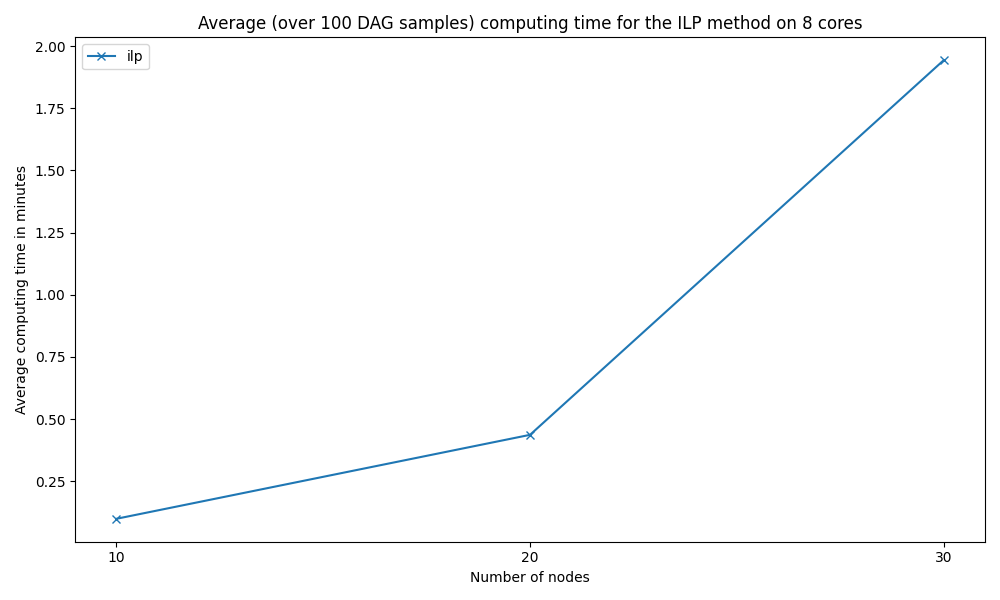
\includegraphics[width=\linewidth]{images/result_computing_time_ilp_m8.png}
    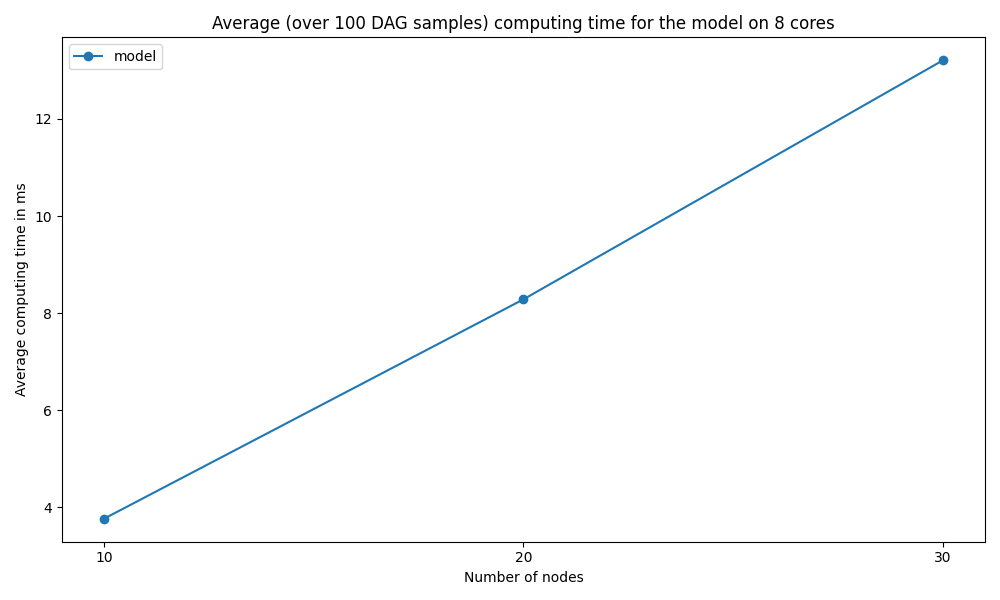
\includegraphics[width=\linewidth]{images/result_computing_time_model_m8.png}
    \caption{Average computing time for computing the optimal schedule
    of a single DAG task using the ILP method (top), in minutes,
    and using the ML model (bottom) according to 
    the number of nodes in the DAG, on a system with 8 cores.}
    \label{fig:compute_time_ilp_model}
\end{figure}

When comparing to the ML model's computing time (Figure \ref{fig:compute_time_ilp_model}),
you can see how, unlike ILP, the model seems to be a lot more scalable
than ILP, as shown by the linearity of the computing time curve (bottom graph of Figure \ref{fig:compute_time_ilp_model}).
The linearity is of course not a true linearity as the theoretical complexity,
in terms of operations on the nodes' vector representation,
of the model can be calculated to be $O(n^2)$ according to Section \ref{sec:model_design},
but the curve is linear because of how short the X axis is,
the polynomial curve is zoomed in which explains why the curve seems linear.

This difference in scalability is expected as the problem is NP-hard,
which means that the ILP solution, calculating optimal solutions,
has to be at least of exponential complexity, hence the non-scalability of the ILP method.
The model's scalability is also expected as the theoritacl complexity
is polynomial.


\subsection{Performance comparison}
~

Two performance metrics will be used for the model.
The makespan which will be compared to the ILP solution, the heuristic
from \citet{zhao2020DAGsched} and a random method where each priority is assigned at random,
and the accuracy / loss of the model.

\begin{figure}
    \centering
    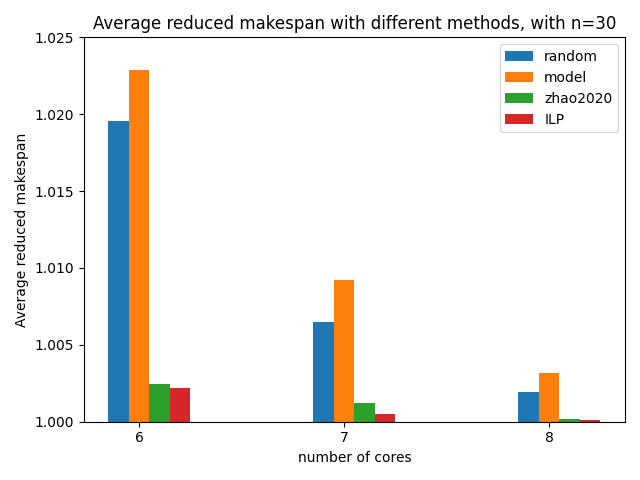
\includegraphics[width=\linewidth]{images/avg_makespan_n30.png}
    \caption{Average reduced makespan (makespan divided by the critical path length) on the test set (400 DAGs) using the four different methods
    on 6, 7 and 8 cores with 30 nodes per DAG,
    with 'random' being the method of randomly assigning priorities to nodes of a DAG.}
    \label{fig:avg_makespan_comparison_trained}
\end{figure}

Figure \ref{fig:avg_makespan_comparison_trained} shows the average
reduced makespan, which is the makespan divided by the length of the critical path,
computed with each method on 400 DAGs from the test set.
Not only does the model perform worse than the heuristic from \citet{zhao2020DAGsched},
the model performs generally worse than the random method.
Also, the heuristic is very close to matching the ILP method,
performing even greater than expected.

When not-trained (Figure \ref{fig:avg_makespan_comparison_untrained}), the model performs 
about the same or slightly worse than randomly, which is expected
given the initialization of trainable weights is done randomly,
confirming the fact that the model's learning decreases its makespan performance.


\begin{figure}
    \centering
    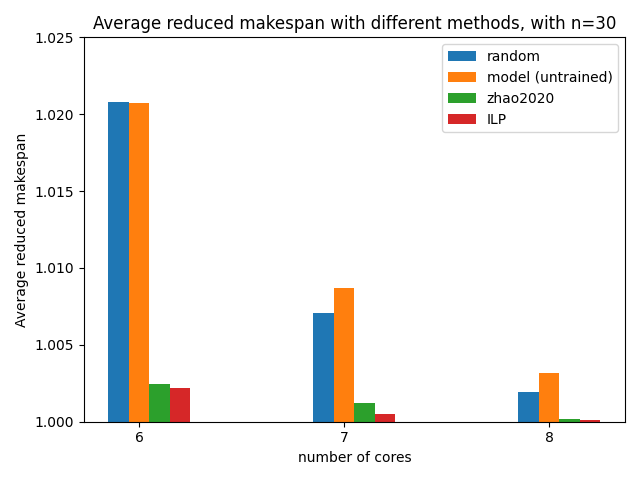
\includegraphics[width=\linewidth]{images/avg_makespan_n30_untrained.png}
    \caption{Average reduced makespan (makespan divided by the critical path length) on the test set (400 DAGs) using the four different methods
    on 6, 7 and 8 cores with 30 nodes per DAG,
    with 'random' being the method of randomly assigning priorities to nodes of a DAG,
    and the model not being trained.}
    \label{fig:avg_makespan_comparison_untrained}
\end{figure}


In terms of accuracy and loss, the results are shown in Figure \ref{fig:accu_loss_model}.
The accuracy is, in this case, how well the resulting priority list 
from the model matches the ILP priority list.
Unfortunately, the accuracy is stagnant at less than 10\%
and doesn't get better when increasing the number of epochs to train on. 
Also, the accuracy doesn't change between the training and testing phase
which further confirms that the model doesn't learn at all.

\begin{figure}
    \centering
    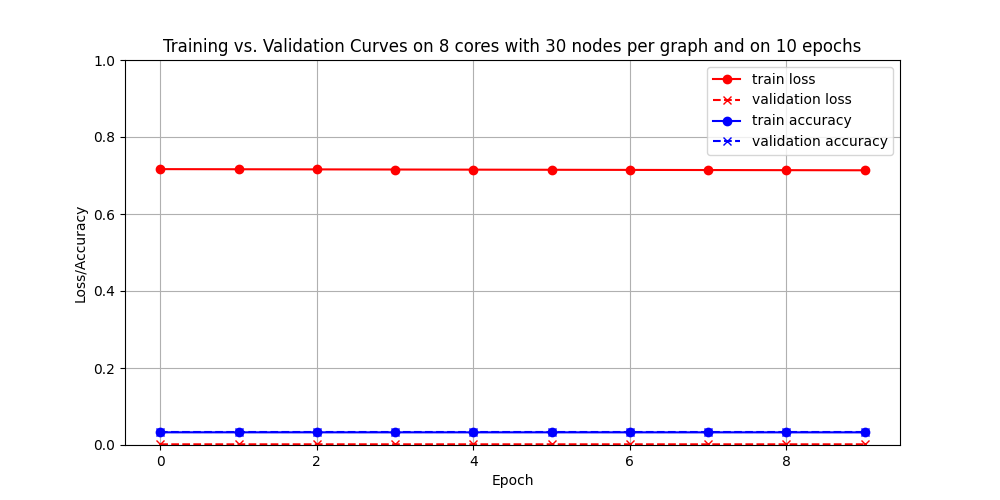
\includegraphics[width=\linewidth]{images/train_val_curves_m8n30epo10.png}
    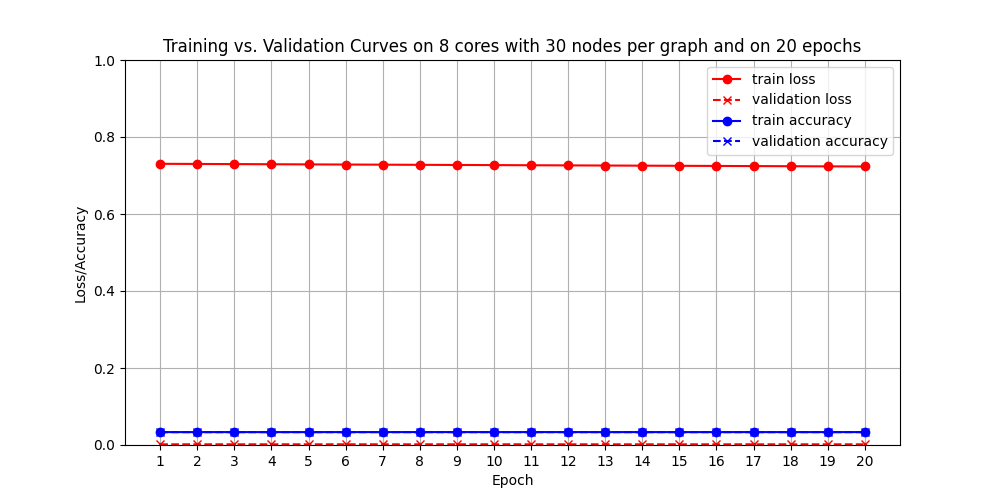
\includegraphics[width=\linewidth]{images/train_val_curves_m8n30epo20.png}
    \caption{Accuracy (in blue) and loss (in red) values for training (circles) and testing (crosses),
    accross the epochs. The top graph shows results for 10 epochs
    and the bottom one for 20 epochs. The results are shown on 8 cores with 30 nodes per DAGs,
    with a training batch size of 250 and a learning rate of $0.001$.}
    \label{fig:accu_loss_model}
\end{figure}

Furthermore,
when looking at the output of the model (Table \ref{tab:similarity_percentages}),
we can see that in most cases,
the priority lists predicted by the model are, on average, more than 90\% 
made out of the same value, i.e., for 10 nodes : [1, 1, 1, 1, 1, 1, 1, 1, 2, 1] for instance.
This shows that the over-smoothing of the DAGs is still an issue for the model and explains
the low accuracy.

\begin{table}
    \begin{tabular}{|c|c|c|c|}
        \hline
        \textbf{number of nodes per DAG/number of cores} & \textbf{6} & \textbf{7} & \textbf{8}\\
        \hline
        \textbf{10} & 94\% & 99\% & 94\%\\
        \hline
        \textbf{20} & 91\% & 60\% & 90\%\\
        \hline
        \textbf{30} & 100\% & 99\% & 98\%\\
        \hline
    \end{tabular}
    \caption{Average percentage of the number of priority slots that have the same value
    in a priority-list outputed by the model.}
    \label{tab:similarity_percentages}
\end{table}


Although the accuracy results shown here are only 
in the case of 8 cores and 30 nodes per DAG,
the other cases, i.e., for 6, 7 cores and with 10,20 and 30 nodes per DAG,
display very similar results and lead to the same conclusions as those
shown here.

\subsection{Discussions}
~

There are several reasons why a machine learning model
sub-performs.
The issue can be because of an overfitting problem,
meaning that the model is too complex and learns the noise / bias
that comes with the dataset.
It can also be the opposite, under-fitting, 
which is due to a model that is too simple for the task at stake,
lacking the architecture to capture the complex information and 
relationships
in the data.
It can be because of the nature of the dataset that is too biased
or too noisy which makes it impossible for the model to learn from it.
Finally, it can be because the model didn't train on enough data 
or on enough epochs, which would mean that the model didn't have
the time to converge and need more data samples to do so.

Let's tackle these different problems and see why 
the problem is the fact that supervised-learning isn't fit for this kind of problem,
that is the single DAG task scheduling problem.


\subsubsection{Biased data and amount of data}
~

Data is always bias and the amount of dataset bias\cite{torralba2011biasdataset}
can have a huge impact on the performance of a model.
Although the number of training samples (1000) is not a lot 
compared to what \citet{Lee2021GlobalDagSchedDRL} have generated (8000),
the dataset generation procedure is the same as the one 
in both \citet{zhao2020DAGsched} and \citet{Lee2021GlobalDagSchedDRL}.
The latter specifically, got more than promising results with their machine learning model,
outperforming the heuristic in \citet{zhao2020DAGsched} by up to 3\% in terms of makespan,
 when using the same data generation procedure as here.
Furthermore, the loss is extremely stable and doesn't go down
during training, even when training on 20 epochs (Figure \ref{fig:accu_loss_model}).
This means that even if there is bias in the data, the fact that others have used
the same data generation procedure and got great results shows that the
dataset bias cannot explain the low performance of the model.
Also, the fact that the model doesn't seem to learn at all with 
its loss being stagnant accross the epochs, removes the 
idea of the model performing badly because there is not enough data to learn on.


\subsubsection{Over-fitting or under-fitting}
~

The reason why the model is performing this badly is probably
not over-fitting.
This is because over-fitting is characterized
by the model learning the noise in the training set and performing\cite{jabbar2015overfitting_underfitting}.
Hence, if it were the case, there would be a noticable gap
between the training and validation accuracy in Figure \ref{fig:accu_loss_model},
which there isn't.
Also, the over-smoothing problem, which is causing the model to sub-perform,
 doesn't come from the noise
in the data but rather from the architecture of the model itself\cite{chen2020oversmoothing}.
Hence the problem might rather be that the model is under-fit for this problem.

Indeed, as mentioned before, what the model is learning is 
to assign the same priority at every node, which also means
that it doesn't learn to approximate the output given by the ILP priority-lists,
as shown by the accuracy and loss values not notably decreasing during
training (Figure \ref{fig:accu_loss_model}).
The issue here is that the model resembles very closely the 
encoder in \citet{Lee2021GlobalDagSchedDRL} which didn't 
have the over-smoothing problem.
The attention-mechanism used is also close to what is done in \citet{Zhao2024GATDRLmodel}
which also didn't have an over-smoothing problem.

The fact that The over-smoothing is very strong (see Table \ref{tab:similarity_percentages})
and that the model is close to what has been done in the reinforcement learning models\cite{Lee2021GlobalDagSchedDRL}\cite{Zhao2024GATDRLmodel},
lead us to conclude that the problem might be the learning method, 
that is the supervised learning method.

\subsubsection{the supervised learning problem}
~

In supervised learning, the problem is either going to be a
regression problem, when dealing with real numbers as the target variable
such as predicting the price of a product or the rate of infection in an epidemic, etc.
Or the problem is going to be interpreted as a classification problem.
In our case, the numbers are discrete and the set of priorities is finite
which is why the problem was treated as a classification problem.
However, usually, for supervised learning, the predicted output 
aim at mathing a ground truth, known beforehand, that is unique.
Although the ILP method permitted us to have a priority list that
effectively yields the minimum makespan,
that priority list is not unique.

Indeed, not only is the minimum makespan schedule not necessarily unique
(see Figure \ref{fig:not_unique_schedules}),
which means that the optimal priority-list is not unique
(in Figure \ref{fig:not_unique_schedules}, schedule a) gives 
[0, 1, 2, 3, 4, 5] but schedule b) gives [0, 1, 2, 4, 3, 5]).
But even if the schedule might be unique, when the start time
of nodes are the same, multiple priorities
can be assigned to those nodes.
For instance, in schedule a) of Figure \ref{fig:not_unique_schedules},
the  two priority-lists [0, 1, 2, 3, 4, 5] and [0, 2, 1, 3, 4, 5]
are valid for minimizing the makespan of the DAG.

\begin{figure}
    \centering
    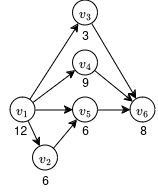
\includegraphics[width=0.5\linewidth]{images/dag_same_makespan_diff_scheds.png}
    \par a)
    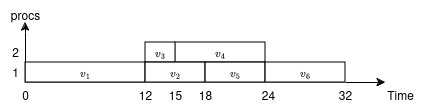
\includegraphics[width=\linewidth]{images/first_samemakespan_diff_sched.png}
    \par b)
    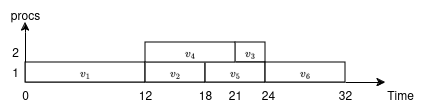
\includegraphics[width=\linewidth]{images/second_samemakespan_diff_sched.png}
    \par c)
    \caption{Example of DAG task (a) for which two schedules (b and c) leading to different
    priority lists are shown, both schedules giving the minimum makespan.}
    \label{fig:not_unique_schedules}    
\end{figure}


This complete lack of uniqueness in the true labels 
renders the ILP priority-lists almost useless
for the model to learn on, because those lists
don't show the difference between a node having 
a specific priority because it lengthen the makespan otherwise (e.g.,
priority of $v_8$ in the last two schedule scenarios in Figure \ref{fig:dag_schedule_example}),
and a node having a specific priority when it could have 
other potential priority values and it wouldn't change the makespan (e.g.,
the example in Figure \ref{fig:not_unique_schedules}).
Thus, the model can't learn to assign different priorities
to the nodes but rather to smooth out the priorities and give
the same one to most of the nodes of a DAG,
hence the over-smoothing problem.\\\\

The evaluation results show that the supervised learning model
doesn't learn correctly, leading to an over-smoothing and under-fitting problem
which makes the model perform very poorly (accuracy $<10$\%)
and having an even worse makespan performance than random priority assignment.
Analysis of the results showed how the model performance problem
is due to the learning method and supervised design being unfit for
the single DAG task fixed-priority scheduling problem.
Thus, relating to RQ3, although the reinforcement learning
method has shown great performance compared to ILP\cite{Zhao2024GATDRLmodel}
and state-of-the-Art heuristics\cite{Lee2021GlobalDagSchedDRL},
the supervised learning model presented here 
clearly cannot compare at all to either SOTA heuristics
or ILP, even though it is more scalable than ILP, 
mostly because of the supervised learning method being unsuited 
for DAG task fixed-priority scheduling.
